\section{DCF i detalj}
\label{sec:dcf}

En kassaflödesvärdering \eng{discounted cash flow, DCF} säger att ett bolag är värt nuvärdet av
alla pengar det kommer att dela ut till sina finansiärer. Resten är bokföring av den meningen.
Det här kapitlet härleder formlerna och visar vid varje steg vad motorn gör, med Atlas Copco
som räkneexempel.

\subsection{Nuvärde}

En krona som placeras till räntan $r$ är värd $(1+r)^t$ kronor om $t$ år. Omvänt är en krona
som betalas om $t$ år värd $(1+r)^{-t}$ kronor i dag. Det är nuvärdet \eng{present value}.
Räntan $r$ ska spegla risken i kassaflödet: den är den avkastning investerarna hade kunnat få
på något annat med samma risk (alternativkostnaden). Ett bolags rörelsevärde är då
\begin{equation}
  \EV = \sum_{t=1}^{\infty} \frac{\FCFF_t}{(1+r)^t}.
  \label{eq:ev-oandlig}
\end{equation}
Ingen kan prognostisera oändligt många år. Därför delar man summan i en uttalad prognosperiod
på $N$ år och ett slutvärde \eng{terminal value} som samlar allt därefter:
\begin{equation}
  \EV = \sum_{t=1}^{N} \frac{\FCFF_t}{(1+r)^t} + \frac{\TV_N}{(1+r)^N}.
  \label{eq:ev}
\end{equation}

\subsection{Prognosen}
\label{sec:prognos}

Motorn prognostiserar $N = 5$ år med fem drivare. Omsättningen växer med $R_t = R_{t-1}(1+g_t)$,
och resten är andelar av omsättningen: $\EBITDA_t = m R_t$, avskrivningar $d R_t$, capex
$c R_t$ och $\Delta\NWC_t = \nu (R_t - R_{t-1})$. Kassaflödet följer av~\eqref{eq:fcff}.
Standardantagandena räknas mekaniskt ur historiken:

\begin{itemize}
  \item \textbf{Tillväxt:} den årliga tillväxttakten \eng{compound annual growth rate, CAGR} över
    de högst fyra senaste boksluten, begränsad till intervallet $-5$ till $+15$\pct, som sedan
    faller linjärt till $g$ år 5.
  \item \textbf{Marginal, avskrivningar, capex och rörelsekapital:} snittet av de tre senaste
    åren, konstant under hela prognosen.
  \item \textbf{Skatt och evig tillväxt:} 20,6\pct{} och 2\pct{} från marknadsparametrarna.
\end{itemize}

\begin{table}[ht]
\centering\small
\caption{Motorns prognos för Atlas Copco med standardantaganden (mdkr). Marginal 26,4\pct,
avskrivningar 5,0\pct, capex 3,4\pct{} och rörelsekapital 25,2\pct{} av omsättningen.}
\label{tab:prognos}
\begin{tabular}{@{}lrrrrr@{}}
\toprule
 & 2026 & 2027 & 2028 & 2029 & 2030 \\
\midrule
Tillväxt & 6,0\pct & 5,0\pct & 4,0\pct & 3,0\pct & 2,0\pct \\
Omsättning & 178,5 & 187,4 & 194,9 & 200,7 & 204,7 \\
EBITDA & 47,1 & 49,5 & 51,4 & 53,0 & 54,0 \\
$-$ Avskrivningar & 9,0 & 9,4 & 9,8 & 10,1 & 10,3 \\
$=$ EBIT & 38,1 & 40,0 & 41,6 & 42,9 & 43,7 \\
$-$ Skatt på EBIT & 7,9 & 8,2 & 8,6 & 8,8 & 9,0 \\
$=$ NOPAT & 30,3 & 31,8 & 33,0 & 34,0 & 34,7 \\
$+$ Avskrivningar & 9,0 & 9,4 & 9,8 & 10,1 & 10,3 \\
$-$ Capex & 6,1 & 6,4 & 6,7 & 6,9 & 7,0 \\
$-$ Ökning av rörelsekapital & 2,5 & 2,2 & 1,9 & 1,5 & 1,0 \\
$=$ \textbf{FCFF} & \textbf{30,6} & \textbf{32,6} & \textbf{34,3} & \textbf{35,8} & \textbf{37,0} \\
\addlinespace
Diskonteringstid, år & 0,5 & 1,5 & 2,5 & 3,5 & 4,5 \\
Diskonteringsfaktor vid 7,65\pct & 0,964 & 0,895 & 0,832 & 0,773 & 0,718 \\
Nuvärde & 29,5 & 29,2 & 28,6 & 27,7 & 26,6 \\
\bottomrule
\end{tabular}
\end{table}

Summan av nuvärdena i tabell~\ref{tab:prognos} är 141,5~mdkr. Att diskonteringstiden är 0,5 och
inte 1 det första året förklaras i avsnitt~\ref{sec:midyear}.

\subsection{Slutvärde med Gordons formel}
\label{sec:gordon}

Anta att kassaflödet efter år $N$ växer med konstant takt $g$ för alltid, så att
$\FCFF_{N+k} = \FCFF_{N+1}(1+g)^{k-1}$. Värdet vid utgången av år $N$ är då en geometrisk serie
med kvoten $q = (1+g)/(1+r)$:
\begin{equation}
  \TV_N = \sum_{k=1}^{\infty} \frac{\FCFF_{N+1}(1+g)^{k-1}}{(1+r)^k}
        = \frac{\FCFF_{N+1}}{1+r} \sum_{j=0}^{\infty} q^{\,j}
        = \frac{\FCFF_{N+1}}{1+r} \cdot \frac{1}{1-q}
        = \frac{\FCFF_{N+1}}{r-g}.
  \label{eq:gordon}
\end{equation}
Serien konvergerar bara om $q < 1$, det vill säga $g < r$. Det är också ekonomiskt rimligt: ett
bolag som för alltid växer snabbare än avkastningskravet blir till slut större än hela
ekonomin. I praktiken sätts $g$ nära den långsiktiga inflationen eller nominella
BNP-tillväxten. Projektet använder 2\pct, Riksbankens inflationsmål.

\begin{komihag}
Formeln~\eqref{eq:gordon} har en pol i $r = g$, och värdet är mycket känsligt nära den:
$\partial \TV / \partial r = -\TV/(r-g)$. För Atlas Copco är $r - g = 5,65$ procentenheter, så
en procentenhet högre WACC sänker slutvärdet med ungefär 15\pct. Motorn vägrar räkna om
$r - g$ är mindre än 0,5 procentenheter.
\end{komihag}

\paragraph{Vilket kassaflöde ska in i täljaren?} Här gör motorn mer än läroboken. Den tar inte
$\FCFF_N (1+g)$ rakt av utan bygger ett normaliserat år $N+1$:
\begin{equation}
  \FCFF_{N+1} = R_N \bigl[(1+g)\,u - \nu g\bigr],
  \qquad u = (m-d)(1-\tau) + d - \max(c, d).
  \label{eq:terminal-fcff}
\end{equation}
Två saker skiljer. Rörelsekapitalet växer bara med $g$ (termen $\nu g$), inte med sista
prognosårets tillväxt. Och capex sätts till minst avskrivningarna, $\max(c, d)$.

\begin{imotorn}
\textbf{Capex-golvet är en avvikelse från standardmodellen.} Tanken är att ett bolag som för
alltid investerar mindre än det skriver av till slut saknar tillgångar. För Atlas Copco är
capex 3,4\pct{} och avskrivningarna 5,0\pct{} av omsättningen, så golvet biter: det sänker
Gordon-värdet från 124,7 till 115,8\kr{} per aktie. Golvet är försiktigt men inte självklart
rätt, eftersom avskrivningarna också innehåller leasade tillgångar och förvärvade immateriella
tillgångar som inte återinvesteras via capex. Det verkar dessutom bara åt ett håll.
\end{imotorn}

För Atlas Copco: $u = 0,2135 \cdot 0,794 + 0,0504 - 0,0504 = 0,1696$ och
$\FCFF_{N+1} = 204,7 \cdot (1,02 \cdot 0,1696 - 0,2516 \cdot 0,02) = 34,4$~mdkr.

\subsection{Slutvärde med exit-multipel}

Den andra metoden antar att bolaget säljs vid utgången av år $N$ till en multipel $M$ av det
årets EBITDA:
\begin{equation}
  \TV_N = M \cdot \EBITDA_N .
  \label{eq:exit}
\end{equation}
Metoden är populär på banker eftersom den är lätt att förklara, men den smyger in en
marknadsvärdering i något som skulle vara en fristående beräkning. I motorn kommer $M$, i
tur och ordning, från ett uttryckligt antagande, från medianen bland jämförelsebolagen (samma
bolag som i kapitel~\ref{sec:multiplar}) eller från bolagets egen multipel i dag. Standardvärdet
begränsas till intervallet 4 till 20 gånger. För Atlas Copco blir det 19,4.

\paragraph{Korskontroll.} De två metoderna ska alltid stämmas av mot varandra, och motorn
rapporterar båda kontrollerna:

\begin{itemize}
  \item \emph{Implicit multipel} \eng{implied exit multiple}: Gordon-slutvärdet delat med
    $\EBITDA_N$. För Atlas Copco $631,1 / 54,0 = 11,7$ gånger.
  \item \emph{Implicit tillväxt} \eng{implied perpetual growth}: det $g$ som får Gordons formel
    att ge exit-metodens slutvärde. I lärobokens form, med
    $\TV = \FCFF_N(1+g)/(r-g)$, blir det $g = (\TV \cdot r - \FCFF_N)/(\TV + \FCFF_N)$.
    Motorn löser samma ekvation för sitt normaliserade kassaflöde~\eqref{eq:terminal-fcff}
    och får 4,3\pct{} för Atlas Copco.
\end{itemize}

Här syns hela caset i miniatyr: jämförelsebolagens multipel 19,4 motsvarar 4,3\pct{} evig
tillväxt, medan modellens 2\pct{} motsvarar multipeln 11,7. Det kan inte båda vara rätt.

\subsection{Halvårskonventionen}
\label{sec:midyear}

Formel~\eqref{eq:ev} låtsas att hela årets kassaflöde kommer den 31 december. I verkligheten
kommer det löpande under året, i genomsnitt vid halvårsskiftet. Halvårskonventionen
\eng{mid-year convention} diskonterar därför kassaflödet för år $t$ med $t - \tfrac12$ år:
\begin{equation}
  \EV = \sum_{t=1}^{N} \frac{\FCFF_t}{(1+r)^{t-1/2}} + \frac{\TV_N}{(1+r)^N}.
  \label{eq:ev-midyear}
\end{equation}
Slutvärdet kräver eftertanke, och de två metoderna ska behandlas olika:

\begin{itemize}
  \item \textbf{Gordon.} Formel~\eqref{eq:gordon} värderar flöden som kommer vid årens slut. Med
    halvårskonventionen kommer även de eviga flödena ett halvår tidigare. Slutvärdet vid
    utgången av år $N$ blir därför $\FCFF_{N+1}/(r-g) \cdot (1+r)^{1/2}$, som sedan diskonteras
    $N$ hela år.
  \item \textbf{Exit-multipel.} En försäljning sker vid ett bestämt datum, utgången av år $N$.
    Slutvärdet diskonteras $N$ hela år och får \emph{ingen} halvårsjustering.
\end{itemize}

Så gör motorn, och koden är kort nog att läsa. Lägg märke till att \kod{mid_year_factor} bara
används på Gordon-raden:

\begin{lstlisting}[caption={Ur \texttt{dcf\_core} i \texttt{models/dcf.py} (förkortat).},label=lst:dcf]
fcff = nopat + da - capex - delta_nwc

periods = np.arange(1, n_years + 1, dtype=float) - (0.5 if mid_year else 0.0)
factors = (1.0 + rate) ** (-periods)
pv_fcff = np.sum(fcff * factors, axis=1, keepdims=True)
end_factor = (1.0 + rate) ** (-float(n_years))  # discount from END of year N

mid_year_factor = (1.0 + rate) ** 0.5 if mid_year else np.ones_like(rate)
spread = rate - g
tv_gordon = np.where(spread > 0, terminal_fcff / spread * mid_year_factor, np.nan)
pv_tv_gordon = tv_gordon * end_factor
ev_gordon = pv_fcff + pv_tv_gordon

tv_exit = multiple * last_ebitda
pv_tv_exit = tv_exit * end_factor
ev_exit = pv_fcff + pv_tv_exit
\end{lstlisting}

För Atlas Copco höjer konventionen Gordon-värdet från 111,6 till 115,8\kr{} per aktie och
exit-värdet från 174,2 till 175,2\kr.

\subsection{WACC: vad kapitalet kostar}
\label{sec:wacc}

FCFF tillhör både långivare och aktieägare, så diskonteringsräntan ska vara ett vägt snitt av
vad de två grupperna kräver. Det är WACC \eng{weighted average cost of capital}:
\begin{equation}
  \WACC = \frac{E}{E+D}\, r_e + \frac{D}{E+D}\, r_d\,(1-\tau).
  \label{eq:wacc}
\end{equation}
Vikterna ska vara marknadsvärden, inte bokförda värden. Faktorn $(1-\tau)$ finns där eftersom
räntan är avdragsgill: varje krona i ränta sänker skatten med $\tau$ kronor, så statens del av
räntan ska inte räknas som en kostnad. Det är så skatteskölden kommer in i en FCFF-värdering.

\paragraph{Avkastningskravet på eget kapital} kommer från CAPM \eng{capital asset pricing model}:
\begin{equation}
  r_e = r_f + \beta_L \cdot \ERP \;(+\; s).
  \label{eq:capm}
\end{equation}
Här är $r_f$ den riskfria räntan, $\ERP$ riskpremien \eng{equity risk premium}, alltså vad
aktiemarknaden väntas ge utöver den riskfria räntan, och $\beta_L$ aktiens känslighet för
marknaden. Tanken är att bara risk som inte går att diversifiera bort ger betalt. Termen $s$
finns inte i CAPM. Det är motorns storlekspremie, se nedan.

\begin{table}[H]
\centering\small
\caption{WACC för Atlas Copco, så som motorn räknar den.}
\label{tab:wacc}
\begin{tabular}{@{}lrl@{}}
\toprule
Komponent & Värde & Källa \\
\midrule
Riskfri ränta $r_f$ & 3,075\pct & Riksbanken, tioårig statsobligation, 2026-11-13 \\
Riskpremie $\ERP$ & 4,23\pct & Damodaran, Sverige, januari 2026 \\
Beta $\beta_L$ & 1,13 & snitt av eget (1,17) och jämförelsebolagens (1,08) \\
Storlekspremie $s$ & 0,00\pct & börsvärde över 20 mdkr \\
Avkastningskrav $r_e$ & 7,84\pct & $3,075 + 1,1275 \cdot 4,23$ \\
\addlinespace
Låneränta före skatt $r_d$ & 3,575\pct & räntekostnad delat med snittskuld, minst $r_f + 0,5$ \\
Låneränta efter skatt & 2,84\pct & $3,575 \cdot (1 - 0,206)$ \\
\addlinespace
Andel eget kapital & 96,2\pct & börsvärde 938 mdkr \\
Andel skuld & 3,8\pct & räntebärande skuld 37,5 mdkr \\
\textbf{WACC} & \textbf{7,65\pct} & $0,962 \cdot 7,84 + 0,038 \cdot 2,84$ \\
\bottomrule
\end{tabular}
\end{table}

Låneräntan uppskattas som senaste årets räntekostnad delat med snittet av de två senaste årens
skuld. För Atlas Copco ger det 2,5\pct, vilket är lägre än statsobligationsräntan och alltså
inte trovärdigt som dagens lånekostnad. Motorn lyfter därför räntan till sitt golv, riskfri
ränta plus 0,5 procentenheter. Med 4\pct{} skuld i kapitalstrukturen spelar det nästan ingen
roll här.

\subsection{Beta}
\label{sec:beta}

\paragraph{Beta som regression.} Beta definieras av den linjära modellen
$R_i = \alpha + \beta R_m + \varepsilon$, där $R_i$ är aktiens och $R_m$ marknadens avkastning
under samma period. Minsta kvadratmetoden \eng{ordinary least squares, OLS} minimerar
$\sum_k (R_{i,k} - \alpha - \beta R_{m,k})^2$. Derivatan med avseende på $\alpha$ ger
$\hat\alpha = \bar R_i - \hat\beta \bar R_m$, och insatt i derivatan med avseende på $\beta$:
\begin{equation}
  \hat\beta = \frac{\sum_k (R_{m,k} - \bar R_m)(R_{i,k} - \bar R_i)}{\sum_k (R_{m,k} - \bar R_m)^2}
            = \frac{\Cov(R_i, R_m)}{\Var(R_m)} .
  \label{eq:beta}
\end{equation}
Förklaringsgraden är korrelationen i kvadrat, $R^2 = \rho_{im}^2$, och säger hur stor del av
aktiens variation som är marknadsrisk. Motorn använder veckoavkastningar under fem år (260
observationer för Atlas Copco) mot indexet OMX Stockholm PI, och kräver minst 52
observationer. För Atlas Copco blir $\hat\beta = 1,26$ med $R^2 = 0,60$.

\paragraph{Blume-justeringen.} Skattade betavärden tenderar att röra sig mot 1 över tiden, dels
för att bolag mognar, dels för att extrema skattningar till en del är mätfel. Blume-justeringen
\eng{Blume adjustment} väger därför in marknadens beta:
\begin{equation}
  \beta_{\text{just}} = \tfrac23\, \hat\beta + \tfrac13 \cdot 1 .
  \label{eq:blume}
\end{equation}
För Atlas Copco: $\tfrac23 \cdot 1,26 + \tfrac13 = 1,17$.

\paragraph{Beta med och utan skuld.} En akties beta beror både på rörelsens risk och på
skuldsättningen. För att låna beta från jämförelsebolag måste man först rensa bort deras
skuldsättning \eng{unlever} och sedan lägga på målbolagets \eng{relever}. Hamadas formel gör
det. Härledningen i korthet: enligt Modigliani och Miller med skatt är ett belånat bolag värt
$E + D = V_U + \tau D$, det obelånade värdet plus värdet av skatteskölden. Beta för en
portfölj är det värdevägda snittet av delarnas beta, så
$\beta_U V_U + \beta_{TS}\,\tau D = \beta_L E + \beta_D D$. Anta att skulden är riskfri och
konstant, så att $\beta_D = \beta_{TS} = 0$. Då är $\beta_U (E + D - \tau D) = \beta_L E$, eller
\begin{equation}
  \beta_L = \beta_U \Bigl[1 + (1-\tau)\frac{D}{E}\Bigr]
  \qquad\Longleftrightarrow\qquad
  \beta_U = \frac{\beta_L}{1 + (1-\tau)\,D/E} .
  \label{eq:hamada}
\end{equation}

\begin{imotorn}
Motorn (1) rensar varje jämförelsebolags råa beta med bolagets egen skuldsättning
enligt~\eqref{eq:hamada}, (2) tar medianen, (3) lägger på målbolagets skuldsättning, (4)
Blume-justerar och (5) tar snittet med bolagets eget Blume-justerade beta. För Atlas Copco:
median utan skuld 1,09, med Atlas Copcos $D/E = 0,04$ blir det 1,13, efter Blume 1,08, och
snittet med det egna 1,17 blir 1,13. Råa betavärden utanför intervallet 0 till 3 kastas som
brus, och det slutliga värdet begränsas till 0,5 till 2,0. Att Blume-justera även
jämförelsebolagens beta och att ta ett rakt snitt är projektets val, inte en standard.
\end{imotorn}

\paragraph{Storlekspremien.} Motorn lägger en premie $s$ på avkastningskravet efter börsvärde:
0\pct{} över 20~mdkr, 0,5\pct{} över 5~mdkr, 1\pct{} över 1~mdkr, 2\pct{} över 200~mkr och 3\pct{}
därunder. Skälet är att regressionsbeta för illikvida småbolag blir för låg, så att ren CAPM
ger mikrobolag lägre avkastningskrav än storbolag. Var ärlig med vad detta är: trappstegen är
modellbyggarens antagande, inte skattade ur data och inte källbelagda. Premien kan stängas av
med flaggan \flag{no-size-premium}. Atlas Copco får 0\pct.

\subsection{Från rörelsevärde till värde per aktie}
\label{sec:brygga}

Rörelsevärdet tillhör alla finansiärer. För att få aktieägarnas del drar man av de andras
anspråk. Den uppställningen kallas bryggan \eng{equity bridge}:
\begin{equation}
  \text{aktievärde} = \EV - {\underbrace{(\text{skuld} - \text{kassa})}_{\text{nettoskuld}}}
    - \text{minoritetsintressen} - \text{preferensaktier}.
  \label{eq:brygga}
\end{equation}
Kassan läggs tillbaka eftersom den inte behövs i rörelsen och inte ingår i FCFF.
Minoritetsintressen \eng{non-controlling interests} dras av eftersom koncernens kassaflöde
räknas till 100\pct{} även för dotterbolag som delvis ägs av andra.

\begin{table}[H]
\centering\small
\caption{Bryggan för Atlas Copco, Gordon-metoden och exit-metoden (mdkr). Talen är avrundade var för sig.}
\label{tab:brygga}
\begin{tabular}{@{}lrr@{}}
\toprule
 & Gordon & Exit-multipel \\
\midrule
Nuvärde av FCFF 2026 till 2030 & 141,5 & 141,5 \\
Slutvärde vid utgången av 2030 & 631,1 & 1\,050,2 \\
Nuvärde av slutvärdet & 436,5 & 726,4 \\
\textbf{Rörelsevärde} & \textbf{578,0} & \textbf{867,8} \\
\quad varav slutvärde & 76\pct & 84\pct \\
$-$ Nettoskuld ($37,5 - 25,1$) & 12,4 & 12,4 \\
$-$ Minoritetsintressen & 0,2 & 0,2 \\
\textbf{Aktievärde} & \textbf{565,4} & \textbf{855,2} \\
Antal aktier, miljoner & 4\,880 & 4\,880 \\
\textbf{Värde per aktie, kr} & \textbf{115,8} & \textbf{175,2} \\
\bottomrule
\end{tabular}
\end{table}

Antalet aktier är börsvärdet delat med kursen. Det hanterar att Atlas Copco har både A- och
B-aktier: Yahoo räknar börsvärdet på alla aktier till det valda aktieslagets kurs.

\subsection{Känslighet}

Eftersom tre fjärdedelar av värdet ligger i slutvärdet ska en DCF alltid visas med en
känslighetstabell. Figur~\ref{fig:dcf-sens} är motorns. En procentenhet lägre WACC och en halv
procentenhet högre tillväxt lyfter värdet från 115,8 till 153,7\kr. Det är just de två hörnen
(och deras motsatser) som blir stapelns ändar i football field: lågt värde är WACC plus 1,0
och $g$ minus 0,5 procentenheter, högt värde tvärtom.

\begin{figure}[ht]
\centering
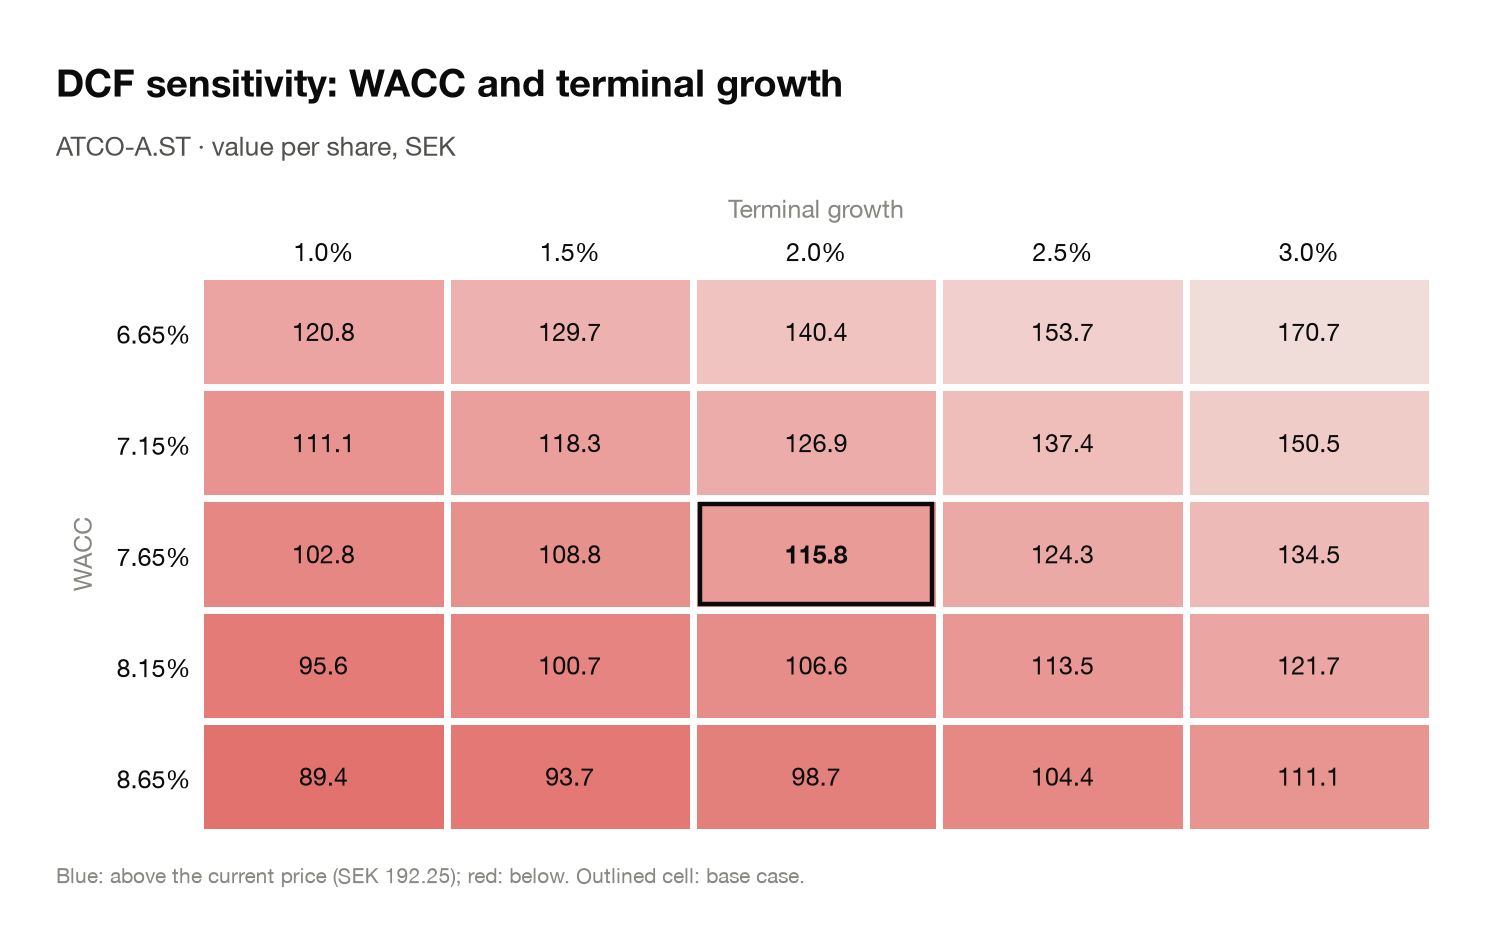
\includegraphics[width=0.8\linewidth]{dcf_sensitivity_wacc_growth.png}
\caption{Värde per aktie för Atlas Copco som funktion av WACC och evig tillväxt. Mittenrutan
är basfallet 115,8\kr.}
\label{fig:dcf-sens}
\end{figure}

\subsection{Vanliga misstag, och motorns egna förenklingar}

\begin{vanligtfel}
\begin{itemize}[leftmargin=1.2em]
  \item Att diskontera FCFF med avkastningskravet på eget kapital, eller FCFE med WACC.
  \item Att halvårsjustera slutvärdet från en exit-multipel, eller glömma justeringen på Gordon.
  \item Att använda bokförda värden som vikter i WACC, eller jämförelsebolagens beta utan att
    först rensa bort deras skuldsättning.
  \item Att sätta $g$ över ekonomins långsiktiga nominella tillväxt.
  \item Att glömma minoritetsintressen, leasingskulder eller pensionsskulder i bryggan.
  \item Att inte kontrollera slutvärdets andel och den implicita multipeln.
\end{itemize}
\end{vanligtfel}

Motorn har också egna förenklingar, och de ska du kunna redogöra för. Det finns ingen
stubbperiod: modellen värderar som om år 1 just hade börjat, fast kursen är från november.
Leasing enligt IFRS~16 gör kassaflödena under prognosåren något för höga. Prognosen är mekanisk
och bygger på högst fyra bokslut. Och tillväxten bromsar till 2\pct{} redan år 5, vilket är
snålt mot ett bolag som marknaden ger en kvalitetspremie.
